\documentclass[12pt, titlepage]{article}
\usepackage[bottom = 3cm, top = 3cm, left = 3cm, right = 3cm]{geometry}
\usepackage[english]{babel}
\usepackage[utf8]{inputenc}
\usepackage[table]{xcolor}
\usepackage{graphicx, booktabs, tikz, csquotes, subfig, enumitem, dcolumn, pdfpages}
\usepackage[font=normalsize]{caption}%,labelfont=bf
\usepackage{subcaption}

\renewcommand*\rmdefault{ppl}

\usepackage{setspace}
\setstretch{1.5}

\usepackage[]{titlesec}
    \titleformat*{\section}{\large\bf}
    \titleformat*{\subsection}{\normalsize\it}

% Bibliography
% \usepackage[natbibapa]{apacite}
\usepackage[round]{natbib}
% \renewcommand{\bibliographytypesize}{\normalsize}
\setlength{\bibsep}{5pt}

\usepackage[colorlinks = TRUE, allcolors = blue]{hyperref}

\widowpenalty=10000
\clubpenalty=10000

\title{\Large Online Appendix for:\\Do TJ policies cause backlash?\\Evidence from street name changes in Spain}
\author{}
% \author{Francisco Villamil\thanks{Juan March Institute--Carlos III University of Madrid, francisco.villamil@uc3m.es} \and Laia Balcells\thanks{Georgetown University, lb1127@georgetown.edu}}
\date{\today}

\begin{document}

\maketitle

\tableofcontents

% Trying

\begin{table}[!htbp] \centering
\caption{Mean comparison municipalities in/out of sample}
\label{tab:ttest_sample}
\small
\begin{tabular}{lcccc}
\\[-1.8ex]\hline
\hline \\[-1.8ex]
\\[-1.8ex]
Party & In sample & Out of sample & Diff In-Out (\%) & P-value \\
\hline \\[-1.8ex]
& \multicolumn{4}{c}{April 2019}\\
PP & 26.72\% & 23.95\% & 2.77 & 0.000*** \\
PSOE & 31.72\% & 28.04\% & 3.68 & 0.000*** \\
VOX & 12.31\% & 9.33\% & 2.97 & 0.000*** \\
\hline \\[-1.8ex]
& \multicolumn{4}{c}{June 2016}\\
PP & 44.42\% & 38.49\% & 5.94 & 0.000*** \\
PSOE & 27.21\% & 23.13\% & 4.08 & 0.000*** \\
VOX & 0.21\% & 0.2\% & 0.01 & 0.650 \\
\hline \\[-1.8ex]
& \multicolumn{4}{c}{December 2015}\\
PP & 40.34\% & 35.26\% & 5.08 & 0.000*** \\
PSOE & 27.86\% & 23.26\% & 4.6 & 0.000*** \\
VOX & 0.23\% & 0.22\% & 0 & 0.796 \\
\hline \\[-1.8ex]
& \multicolumn{4}{c}{November 2011}\\
PP & 54.87\% & 47.07\% & 7.8 & 0.000*** \\
PSOE & 31.23\% & 28.01\% & 3.23 & 0.000*** \\
\hline
\hline \\[-1.8ex]
\multicolumn{5}{c}{\parbox[t]{0.65\textwidth}{\textit{Note:} + $p<0.1$; * $p<0.05$; ** $p<0.01$; *** $p<0.001$.}}\\
\end{tabular}
\end{table}


\begin{table}[!htbp] \centering
\caption{Mean comparison municipalities with/without Francoist street names in June 2001}
\label{tab:ttest_sample2001}
\small
\begin{tabular}{lcccc}
\\[-1.8ex]\hline
\hline \\[-1.8ex]
\\[-1.8ex]
Party & In sample & Out of sample & Diff In-Out (\%) & P-value \\
\hline \\[-1.8ex]
& \multicolumn{4}{c}{April 2019}\\
PP & 27.23\% & 23.47\% & 3.75 & 0.000*** \\
PSOE & 31.53\% & 27.75\% & 3.77 & 0.000*** \\
VOX & 12.22\% & 9.08\% & 3.15 & 0.000*** \\
\hline \\[-1.8ex]
& \multicolumn{4}{c}{June 2016}\\
PP & 44.85\% & 37.74\% & 7.11 & 0.000*** \\
PSOE & 26.9\% & 22.86\% & 4.04 & 0.000*** \\
VOX & 0.21\% & 0.2\% & 0.02 & 0.278 \\
\hline \\[-1.8ex]
& \multicolumn{4}{c}{December 2015}\\
PP & 40.85\% & 34.57\% & 6.28 & 0.000*** \\
PSOE & 27.5\% & 22.95\% & 4.55 & 0.000*** \\
VOX & 0.24\% & 0.22\% & 0.02 & 0.260 \\
\hline \\[-1.8ex]
& \multicolumn{4}{c}{November 2011}\\
PP & 55.17\% & 46.2\% & 8.96 & 0.000*** \\
PSOE & 31\% & 27.78\% & 3.21 & 0.000*** \\
\hline \\[-1.8ex]
& \multicolumn{4}{c}{March 2008}\\
PP & 48.65\% & 41.07\% & 7.58 & 0.000*** \\
PSOE & 42.99\% & 39.63\% & 3.37 & 0.000*** \\
\hline \\[-1.8ex]
& \multicolumn{4}{c}{March 2004}\\
PP & 48.49\% & 41.57\% & 6.92 & 0.000*** \\
PSOE & 42.09\% & 36.68\% & 5.41 & 0.000*** \\
\hline \\[-1.8ex]
& \multicolumn{4}{c}{March 2000}\\
PP & 53.18\% & 46.81\% & 6.37 & 0.000*** \\
PSOE & 36.21\% & 31.46\% & 4.74 & 0.000*** \\
\hline
\hline \\[-1.8ex]
\multicolumn{5}{c}{\parbox[t]{0.65\textwidth}{\textit{Note:} * $p<0.05$; ** $p<0.01$; *** $p<0.001$.}}\\
\end{tabular}
\end{table}



\section{Francoist street names}

We considered as Francoist the following street names. The starting point was the list published by the Madrid City Council in 2017, where they proposed a list of 52 street names to be removed, following a report by the Historical Memory Commission.\footnote{The full list and the reasons for the choice of each street name is available online at https://bit.ly/37cLGgk (accessed 26/11/2020).}
This list was expanded, manually selecting from the street names most commonly changed.
Indeed, among all the changes between 2001 and 2020, the five most commonly removed street names were all key Francoist figures: `Jose Antonio,' `Calvo Sotelo,' `General Mola,' `Generalísimo,' and `General Franco.'

\begin{quote}
  18 de Julio; Alcalde Conde de Mayalde; Alcazar; Alcazar de Toledo; Alferez Provisional; Almirante Francisco Moreno; Angel del Alcazar; Arco de la Victoria; Arriba Espana; Aunos; Batalla de Belchite; Batalla del Ebro; Caidos; Caidos (de Los); Caidos (los); Caidos de la Division Azul; Caidos Por la Patria; Calvo Sotelo; Calvo Sotelo (de); Capita Cortes; Capitan Cortes; Capitan Cortes (del); Capitan Haya; Capitan Luna; Carlos Pinilla; Carlos Ruiz; Carrero Blanco; Caudillo; Caudillo (del); Cerro de Garabitas; Cirilo Martin Martin; Comandante Franco; Comandante Franco; Comandante Zorita; Conde Vallellano; Crucero Baleares; Defensores del Alcazar; Defensores del Alcazar; Dieciocho de Julio; Diego Salas Pombo; Division Azul; Doctor Vallejo-Nagera; Eduardo Aunos; Ejercito Espanol; El Algabeno; Emilio Jimenez Millas; Falange Espanola; Federico Mayo; Federico Servet; Fernandez Ladreda; Francisco Franco; Franco; Garcia Morato; General; General Aranda; General Asensio Cabanillas; General Cabanellas; General Cabanellas; General Davila; General Fanjul; General Franco; General Garcia de la Herranz; General Garcia Escamez; General Kirkpatrick; General Millan Astray; General Mola; General Mola (del); General Moscardo; General Munoz Grandes; General Orgaz; General Primo de Rivera; General Queipo de Llano; General Rodrigo; General Romero Basart; General Sagardia Ramos; General Saliquet; General Sanjurjo; General Varela; General Yague; Generalisimo; Generalisimo (del); Generalisimo Franco; Gobernador Carlos Ruiz; Hermanos Falco y Alvarez de Toledo; Hermanos Garcia Noblejas; Heroes del Alcazar; Jose Antonio; Jose Antonio (de); Jose Antonio Giron; Jose Antonio Giron; Jose Antonio Primo de Rivera; Jose Luis de Arrese; Jose Maria Peman; Juan Pujol; Juan Vigon; Lepanto; Los Martires; Manuel Sarrion; Martires; Martires (los); Matias Montero; Millan Astray; Munoz Grandes; Onesimo Redondo; Pilar Primo de Rivera; Primero de Octubre; Primo de Rivera; Puerto de los Leones; Queipo de Llano; Ramiro Ledesma; Ramon Franco; Ruiz de Alda; Salas Pombo; Veintiocho de Marzo

\end{quote}

\section{Francoist street name removals}

Figure~\ref{fig:changes_by_prov} shows the number of Francoist street name removals by province in three different time periods: 2001--2020, 2011--2016, and 2016--2018.
Figure~\ref{fig:fs_by_prov} shows the share of Francoist street by province at three different points in time: June 2001, January 2010, and June 2016.

\begin{figure*}[htb!]
\centering

  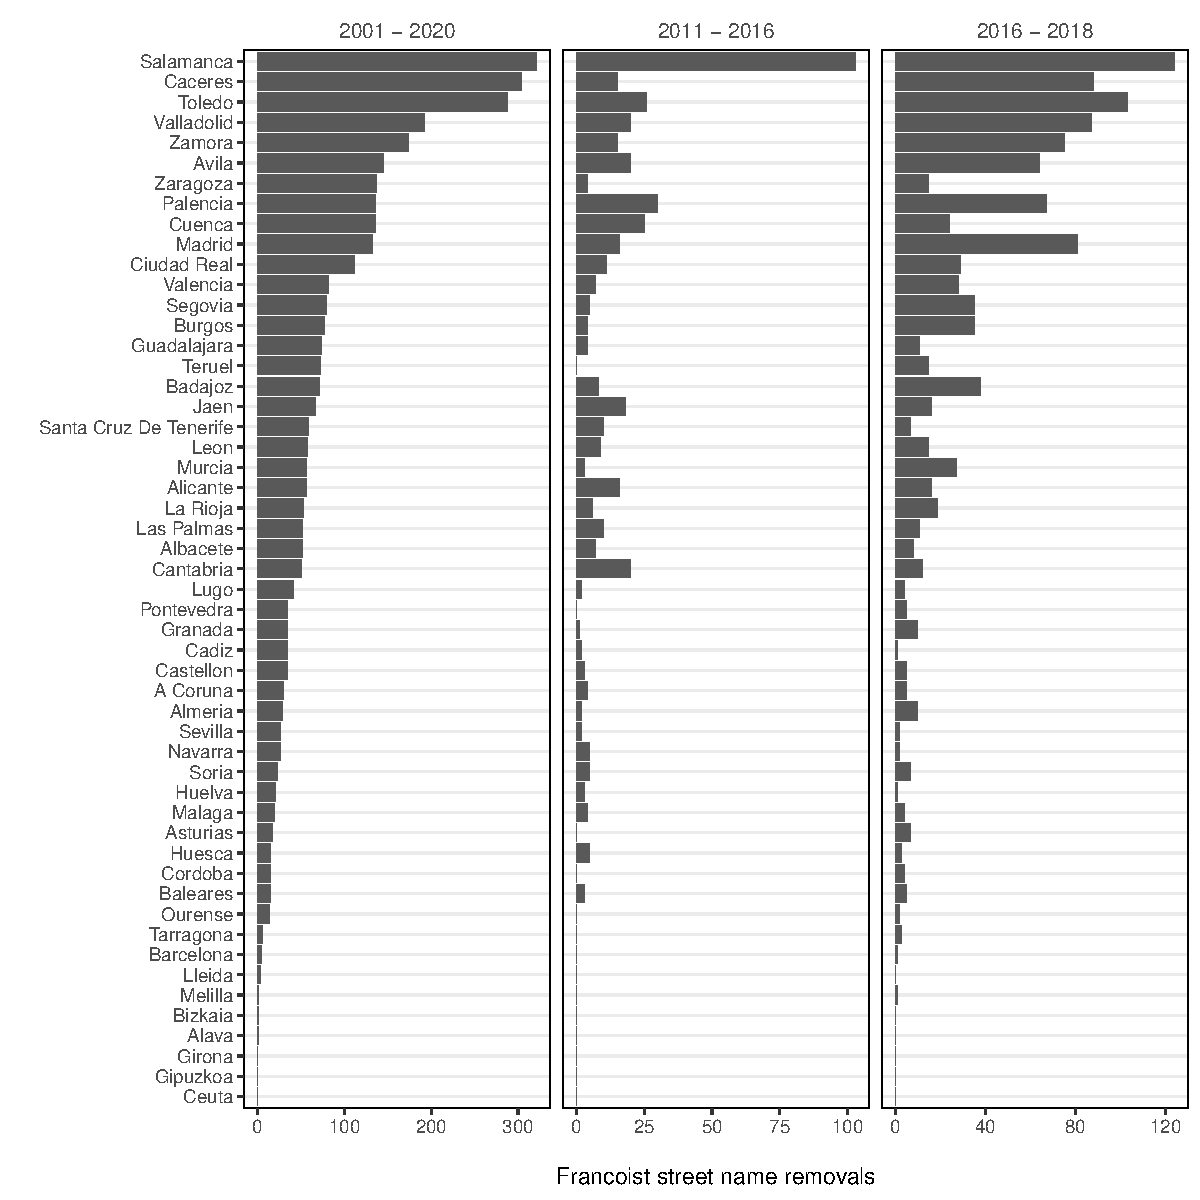
\includegraphics[width = \textwidth]{img/changes_by_prov}

  \caption{Number of Francoist street name removals over time}\label{fig:changes_by_prov}

\end{figure*}

\begin{figure*}[htb!]
\centering

  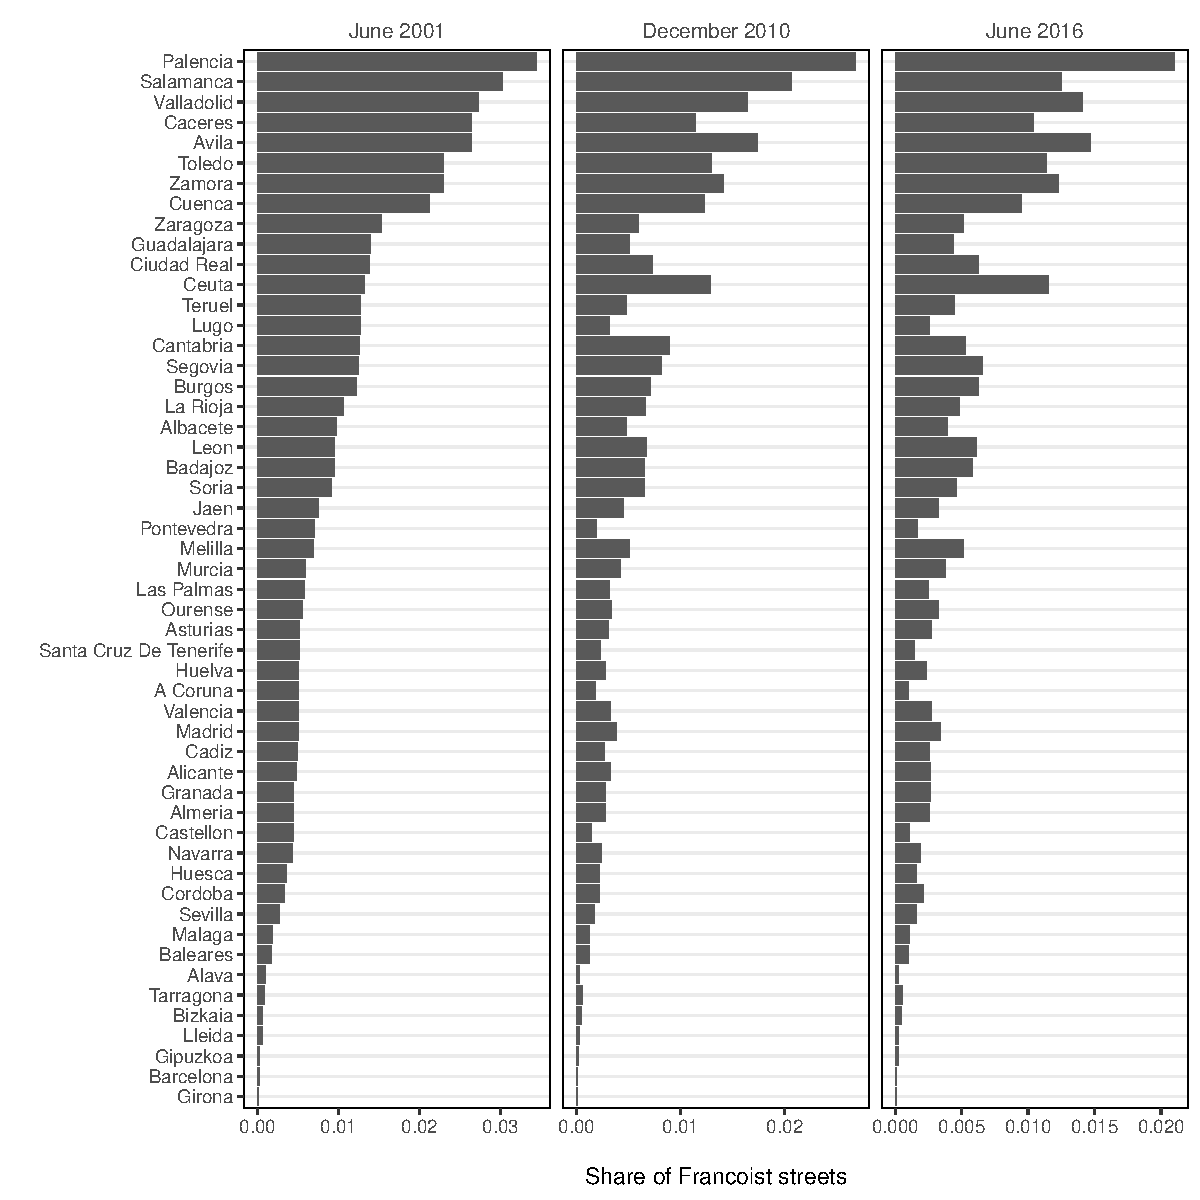
\includegraphics[width = \textwidth]{img/fs_by_prov}

  \caption{Share of Francoist streets in each province}\label{fig:fs_by_prov}

\end{figure*}

Table~\ref{tab:logit_fs_rm} shows the results of regressing a binary indicator of Francoist street name removal between 2016 and 2018 (the period covered in the DiD analyses in the main text) on a set of explanatory variable.
The sample only includes those municipalities that still had Francoist streets in June 2016.
The picture that emerges from these analyses is that it was mainly smaller municipalities with a high number of Francoist streets at the beginning of the period the ones that were more likely to remove Francoist street names.
Moreover, following figures~\ref{fig:changes_by_prov} and \ref{fig:fs_prov_time}, these municipalities were located mostly in the center of Spain.
These results are in line with the idea that municipalities that still had and changed street names during this period were probably the ones that had not done so because of political inaction and that, if anything, the selection bias goes against our main hypothesis.


% Table created by stargazer v.5.2.2 by Marek Hlavac, Harvard University. E-mail: hlavac at fas.harvard.edu
% Date and time: Tue, May 25, 2021 - 13:24:46
% Requires LaTeX packages: dcolumn 
\begin{table}[!htbp] \centering 
  \caption{Logit regression on Francoist street name removal (2016--2018)} 
  \label{tab:logit_fs_rm} 
\small 
\begin{tabular}{@{\extracolsep{-20pt}}lD{.}{.}{-3} D{.}{.}{-3} D{.}{.}{-3} } 
\\[-1.8ex]\hline 
\hline \\[-1.8ex] 
\\[-1.8ex] & \multicolumn{1}{c}{fs\_rm\_2016s2\_2018s2\_bin} & \multicolumn{1}{c}{fs\_rm\_2016s2\_2018s2\_bin} & \multicolumn{1}{c}{fs\_rm\_2016s2\_2018s2\_bin} \\ 
\\[-1.8ex] & \multicolumn{1}{c}{(1)} & \multicolumn{1}{c}{(2)} & \multicolumn{1}{c}{(3)}\\ 
\hline \\[-1.8ex] 
 (Intercept) & 0.326^{***} & 0.150^{*} & -0.289 \\ 
  & (0.044) & (0.062) & (0.206) \\ 
  Leftist mayor 2015 & -0.008 & 0.021 & 0.024 \\ 
  & (0.021) & (0.022) & (0.026) \\ 
  Log. Population 2011 & -0.051^{***} & -0.038^{***} & -0.030^{***} \\ 
  & (0.005) & (0.006) & (0.008) \\ 
  Log. No. Francoist streets June 2016 & 0.339^{***} & 0.328^{***} & 0.342^{***} \\ 
  & (0.023) & (0.024) & (0.027) \\ 
  PP support, June 2016 &  &  & 0.159 \\ 
  &  &  & (0.130) \\ 
  Vox support, June 2016 &  &  & -2.861 \\ 
  &  &  & (3.558) \\ 
  Turnout, June 2016 &  &  & 0.438^{+} \\ 
  &  &  & (0.229) \\ 
 \hline \\[-1.8ex] 
CCAA Fixed Effects & \multicolumn{1}{c}{No} & \multicolumn{1}{c}{Yes} & \multicolumn{1}{c}{Yes} \\ 
Observations & \multicolumn{1}{c}{1,636} & \multicolumn{1}{c}{1,636} & \multicolumn{1}{c}{1,167} \\ 
Log Likelihood & \multicolumn{1}{c}{-867.939} & \multicolumn{1}{c}{-841.697} & \multicolumn{1}{c}{-523.509} \\ 
Akaike Inf. Crit. & \multicolumn{1}{c}{1,743.879} & \multicolumn{1}{c}{1,727.394} & \multicolumn{1}{c}{1,091.019} \\ 
\hline 
\hline \\[-1.8ex] 
\multicolumn{4}{c}{\parbox[t]{0.75\textwidth}{\textit{Note:} + $p<0.1$; * $p<0.05$; ** $p<0.01$; *** $p<0.001$. Only including municipalities that had at least one street with Francoist names in June 2016.}} \\ 
\end{tabular} 
\end{table} 


\section{Additional analysis (cross-sectional)}


% Table created by stargazer v.5.2.2 by Marek Hlavac, Harvard University. E-mail: hlavac at fas.harvard.edu
% Date and time: Wed, Oct 06, 2021 - 13:08:27
% Requires LaTeX packages: dcolumn 
\begin{table}[!htbp] \centering 
  \caption{Francoist street name removal and change in electoral support for Vox during 2019} 
  \label{tab:cs_change} 
\small 
\begin{tabular}{@{\extracolsep{-20pt}}lD{.}{.}{-3} D{.}{.}{-3} } 
\\[-1.8ex]\hline 
\hline \\[-1.8ex] 
\\[-1.8ex] & \multicolumn{1}{c}{\footnotesize Full sample} & \multicolumn{1}{c}{\footnotesize Limited sample} \\ 
\\[-1.8ex] & \multicolumn{1}{c}{(1)} & \multicolumn{1}{c}{(2)}\\ 
\hline \\[-1.8ex] 
 (Intercept) & 2.195^{***} & 2.362^{***} \\ 
  & (0.119) & (0.156) \\ 
  Francoist street name removal & -0.015 & 0.003 \\ 
  & (0.020) & (0.019) \\ 
  Unemployment 2019 & 0.518 & 0.450 \\ 
  & (0.337) & (0.404) \\ 
  Turnout April 2019 & -0.623^{***} & -0.799^{***} \\ 
  & (0.133) & (0.178) \\ 
  Turnout Nov 2019 & -0.009^{+} & -0.018^{**} \\ 
  & (0.005) & (0.006) \\ 
 \hline \\[-1.8ex] 
CCAA Fixed Effects & \multicolumn{1}{c}{Yes} & \multicolumn{1}{c}{Yes} \\ 
Observations & \multicolumn{1}{c}{7,552} & \multicolumn{1}{c}{2,153} \\ 
R$^{2}$ & \multicolumn{1}{c}{0.078} & \multicolumn{1}{c}{0.134} \\ 
Adjusted R$^{2}$ & \multicolumn{1}{c}{0.075} & \multicolumn{1}{c}{0.125} \\ 
\hline 
\hline \\[-1.8ex] 
\multicolumn{3}{c}{\parbox[t]{0.6\textwidth}{\textit{Note:} $+ p<0.1; * p<0.05; ** p<0.01; *** p<0.001$. The main independent variable refers to the removal of Francoist street names between June 2001 and December 2018. The limited sample corresponds to municipalities that had Francoist street names in June 2001.}} \\ 
\end{tabular} 
\end{table} 


Tables~\ref{tab:cs_all_2011} and \ref{tab:cs_limited_2011} replicate the analyses in the main text---plus the model using the change between April and November as dependent variable---using as independent variable the removal of Francoist streets between 2011 and 2018, using the full and limited samples, respectively.


% Table created by stargazer v.5.2.2 by Marek Hlavac, Harvard University. E-mail: hlavac at fas.harvard.edu
% Date and time: Fri, Jun 11, 2021 - 14:03:35
% Requires LaTeX packages: dcolumn 
\begin{table}[!htbp] \centering 
  \caption{Electoral support for Vox and Francoist street name removal (2011--2018)} 
  \label{tab:cs_all_2011} 
\small 
\begin{tabular}{@{\extracolsep{-20pt}}lD{.}{.}{-3} D{.}{.}{-3} D{.}{.}{-3} } 
\\[-1.8ex]\hline 
\hline \\[-1.8ex] 
\\[-1.8ex] & \multicolumn{1}{c}{\footnotesize Apr 2019} & \multicolumn{1}{c}{\footnotesize Nov 2019} & \multicolumn{1}{c}{\footnotesize Change} \\ 
\\[-1.8ex] & \multicolumn{1}{c}{(1)} & \multicolumn{1}{c}{(2)} & \multicolumn{1}{c}{(3)}\\ 
\hline \\[-1.8ex] 
 (Intercept) & 0.078^{***} & 0.145^{***} & 2.197^{***} \\ 
  & (0.009) & (0.010) & (0.119) \\ 
  Francoist street name removal & 0.010^{***} & 0.013^{***} & -0.011 \\ 
  & (0.002) & (0.002) & (0.026) \\ 
  Unemployment 2019 & 0.083^{***} & 0.195^{***} & 0.517 \\ 
  & (0.025) & (0.031) & (0.337) \\ 
  Turnout April 2019 & 0.005 &  & -0.623^{***} \\ 
  & (0.010) &  & (0.133) \\ 
  Turnout Nov 2019 &  & -0.037^{***} &  \\ 
  &  & (0.011) &  \\ 
  Log. Population & 0.003^{***} & 0.006^{***} & -0.009^{+} \\ 
  & (0.000) & (0.000) & (0.005) \\ 
 \hline \\[-1.8ex] 
CCAA Fixed Effects & \multicolumn{1}{c}{Yes} & \multicolumn{1}{c}{Yes} & \multicolumn{1}{c}{Yes} \\ 
Observations & \multicolumn{1}{c}{7,819} & \multicolumn{1}{c}{7,820} & \multicolumn{1}{c}{7,552} \\ 
R$^{2}$ & \multicolumn{1}{c}{0.441} & \multicolumn{1}{c}{0.499} & \multicolumn{1}{c}{0.078} \\ 
Adjusted R$^{2}$ & \multicolumn{1}{c}{0.440} & \multicolumn{1}{c}{0.497} & \multicolumn{1}{c}{0.075} \\ 
\hline 
\hline \\[-1.8ex] 
\multicolumn{4}{c}{\parbox[t]{0.7\textwidth}{\textit{Note:} $+ p<0.1; * p<0.05; ** p<0.01; *** p<0.001$. The main independent variable refers to the removal of Francoist street names between December 2010 and December 2018.}} \\ 
\end{tabular} 
\end{table} 


% Table created by stargazer v.5.2.2 by Marek Hlavac, Harvard University. E-mail: hlavac at fas.harvard.edu
% Date and time: Tue, May 25, 2021 - 14:21:10
% Requires LaTeX packages: dcolumn 
\begin{table}[!htbp] \centering 
  \caption{Electoral support for Vox and Francoist street name removal} 
  \label{tab:cs_limited_2011} 
\small 
\begin{tabular}{@{\extracolsep{-20pt}}lD{.}{.}{-3} D{.}{.}{-3} D{.}{.}{-3} } 
\\[-1.8ex]\hline 
\hline \\[-1.8ex] 
\\[-1.8ex] & \multicolumn{1}{c}{\footnotesize Apr 2019} & \multicolumn{1}{c}{\footnotesize Nov 2019} & \multicolumn{1}{c}{\footnotesize Change} \\ 
\\[-1.8ex] & \multicolumn{1}{c}{(1)} & \multicolumn{1}{c}{(2)} & \multicolumn{1}{c}{(3)}\\ 
\hline \\[-1.8ex] 
 (Intercept) & 0.115^{***} & 0.218^{***} & 2.476^{***} \\ 
  & (0.020) & (0.022) & (0.174) \\ 
  Francoist street name removal & 0.006^{*} & 0.007^{*} & -0.012 \\ 
  & (0.002) & (0.003) & (0.022) \\ 
  Unemployment 2019 & 0.002 & 0.097 & 0.381 \\ 
  & (0.051) & (0.062) & (0.443) \\ 
  Turnout April 2019 & -0.012 &  & -0.901^{***} \\ 
  & (0.023) &  & (0.200) \\ 
  Turnout Nov 2019 &  & -0.088^{***} &  \\ 
  &  & (0.025) &  \\ 
  Log. Population & 0.002^{*} & 0.003^{***} & -0.023^{**} \\ 
  & (0.001) & (0.001) & (0.007) \\ 
 \hline \\[-1.8ex] 
CCAA Fixed Effects & \multicolumn{1}{c}{Yes} & \multicolumn{1}{c}{Yes} & \multicolumn{1}{c}{Yes} \\ 
Observations & \multicolumn{1}{c}{1,791} & \multicolumn{1}{c}{1,792} & \multicolumn{1}{c}{1,782} \\ 
R$^{2}$ & \multicolumn{1}{c}{0.269} & \multicolumn{1}{c}{0.296} & \multicolumn{1}{c}{0.129} \\ 
Adjusted R$^{2}$ & \multicolumn{1}{c}{0.260} & \multicolumn{1}{c}{0.287} & \multicolumn{1}{c}{0.118} \\ 
\hline 
\hline \\[-1.8ex] 
\multicolumn{4}{c}{\parbox[t]{0.7\textwidth}{\textit{Note:} $+ p<0.1; * p<0.05; ** p<0.01; *** p<0.001$. The main independent variable refers to the removal of Francoist street names between December 2010 and December 2018. Only municipalities that had Francoist street names in June 2011 were included.}} \\ 
\end{tabular} 
\end{table} 


\section{Robustness tests (difference-in-differences)}

Table~\ref{tab:vox_robustness} shows the robustness tests for the DiD analyses using electoral support for Vox as the dependent variable, which table~\ref{tab:pp_robustness} does the same but using PP share as the dependent variable.
All models in these tables include elections before June 2016: December 2015 in the case of Vox, and both December 2015 and November 2011 in the case of PP.
Model 2 extends the dependent variable to the first half of 2019, accounting for potential delays in the registration of name changes.
Model 3 uses the independent variable in continuous form, namely, the logged number of changes.
Model 4 restricts the sample to municipalities where Vox got more than 0 votes in 2016 elections.


% Table created by stargazer v.5.2.2 by Marek Hlavac, Harvard University. E-mail: hlavac at fas.harvard.edu
% Date and time: Thu, May 27, 2021 - 19:57:41
% Requires LaTeX packages: dcolumn 
\begin{table}[!htbp] \centering 
  \caption{Francoist street name removal and increase in electoral support for Vox} 
  \label{tab:vox_robustness} 
\small 
\begin{tabular}{@{\extracolsep{-20pt}}lD{.}{.}{-3} D{.}{.}{-3} D{.}{.}{-3} D{.}{.}{-3} } 
\\[-1.8ex]\hline 
\hline \\[-1.8ex] 
\\[-1.8ex] & \multicolumn{1}{c}{(1)} & \multicolumn{1}{c}{(2)} & \multicolumn{1}{c}{(3)} & \multicolumn{1}{c}{(4)}\\ 
\hline \\[-1.8ex] 
 (Intercept) & -0.968^{**} & -0.969^{**} & -0.929^{**} & 0.127 \\ 
  & (0.326) & (0.326) & (0.324) & (0.399) \\ 
  Francoist street name removal & -0.078 & -0.066 & -0.163 & -0.231 \\ 
  & (0.220) & (0.215) & (0.188) & (0.253) \\ 
  Election December 2015 & -0.101 & -0.102 & -0.109 & -0.119 \\ 
  & (0.148) & (0.149) & (0.144) & (0.159) \\ 
  Election April 2019 & 12.319^{***} & 12.305^{***} & 12.300^{***} & 12.898^{***} \\ 
  & (0.142) & (0.144) & (0.139) & (0.153) \\ 
  Francoist removal $\times$ Dec 2015 & -0.019 & -0.011 & 0.021 & -0.048 \\ 
  & (0.314) & (0.306) & (0.253) & (0.362) \\ 
  Francoist removal $\times$ April 2019 & 0.724^{*} & 0.735^{*} & 0.746^{**} & 0.789^{*} \\ 
  & (0.299) & (0.293) & (0.244) & (0.347) \\ 
 \hline \\[-1.8ex] 
Controls & \multicolumn{1}{c}{Yes} & \multicolumn{1}{c}{Yes} & \multicolumn{1}{c}{Yes} & \multicolumn{1}{c}{Yes} \\ 
CCAA Fixed Effects & \multicolumn{1}{c}{Yes} & \multicolumn{1}{c}{Yes} & \multicolumn{1}{c}{Yes} & \multicolumn{1}{c}{Yes} \\ 
Observations & \multicolumn{1}{c}{3,303} & \multicolumn{1}{c}{3,303} & \multicolumn{1}{c}{3,303} & \multicolumn{1}{c}{2,259} \\ 
R$^{2}$ & \multicolumn{1}{c}{0.802} & \multicolumn{1}{c}{0.802} & \multicolumn{1}{c}{0.802} & \multicolumn{1}{c}{0.844} \\ 
Adjusted R$^{2}$ & \multicolumn{1}{c}{0.801} & \multicolumn{1}{c}{0.801} & \multicolumn{1}{c}{0.801} & \multicolumn{1}{c}{0.843} \\ 
\hline 
\hline \\[-1.8ex] 
\multicolumn{5}{c}{\parbox[t]{0.85\textwidth}{\textit{Note:} + $p<0.1$; * $p<0.05$; ** $p<0.01$; *** $p<0.001$. All models also include elections before June 2016 (December 2015). Model 2 extends the DV (name removal) to the first half of 2019. Model 3 uses the IV in continuous form (logged number of changes). Model 4 restricts the sample to municipalities where Vox got more than 0 votes. Controls include a dummy for a leftist major elected in 2015 local elections, logged population in 2011, logged number of Francoist streets in $t_{0}$, and the unemployment rate in January 2016. Only municipalities that had at least one street with a Francoist name in $t_{0}$ (June 2016) were included in the sample.}} \\ 
\end{tabular} 
\end{table} 


% Table created by stargazer v.5.2.2 by Marek Hlavac, Harvard University. E-mail: hlavac at fas.harvard.edu
% Date and time: Tue, Jun 15, 2021 - 19:16:26
% Requires LaTeX packages: dcolumn 
\begin{table}[!htbp] \centering 
  \caption{Francoist street name removal and change in electoral support for PP} 
  \label{tab:pp_robustness} 
\small 
\begin{tabular}{@{\extracolsep{-20pt}}lD{.}{.}{-3} D{.}{.}{-3} D{.}{.}{-3} D{.}{.}{-3} } 
\\[-1.8ex]\hline 
\hline \\[-1.8ex] 
\\[-1.8ex] & \multicolumn{1}{c}{(1)} & \multicolumn{1}{c}{(2)} & \multicolumn{1}{c}{(3)} & \multicolumn{1}{c}{(4)}\\ 
\hline \\[-1.8ex] 
 (Intercept) & 49.323^{***} & 49.312^{***} & 49.484^{***} & 43.384^{***} \\ 
  & (0.593) & (0.594) & (0.589) & (0.751) \\ 
  Francoist street name removal & 1.009^{*} & 0.974^{+} & 0.841^{+} & 0.634 \\ 
  & (0.511) & (0.502) & (0.436) & (0.695) \\ 
  Election March 2000 & 8.091^{***} & 8.015^{***} & 8.132^{***} & 8.539^{***} \\ 
  & (0.374) & (0.379) & (0.363) & (0.428) \\ 
  Election March 2004 & 3.291^{***} & 3.273^{***} & 3.310^{***} & 3.614^{***} \\ 
  & (0.374) & (0.379) & (0.363) & (0.428) \\ 
  Election March 2008 & 4.267^{***} & 4.264^{***} & 4.218^{***} & 6.074^{***} \\ 
  & (0.374) & (0.379) & (0.363) & (0.428) \\ 
  Election November 2011 & 10.569^{***} & 10.561^{***} & 10.538^{***} & 12.127^{***} \\ 
  & (0.374) & (0.379) & (0.363) & (0.428) \\ 
  Election December 2015 & -4.075^{***} & -4.063^{***} & -4.039^{***} & -4.218^{***} \\ 
  & (0.374) & (0.379) & (0.363) & (0.428) \\ 
  Election April 2019 & -17.382^{***} & -17.343^{***} & -17.379^{***} & -17.657^{***} \\ 
  & (0.376) & (0.381) & (0.364) & (0.428) \\ 
  Francoist removal $\times$ March 2000 & -0.106 & 0.161 & -0.241 & 0.132 \\ 
  & (0.711) & (0.698) & (0.594) & (0.970) \\ 
  Francoist removal $\times$ March 2004 & 0.741 & 0.754 & 0.634 & 0.674 \\ 
  & (0.711) & (0.697) & (0.594) & (0.970) \\ 
  Francoist removal $\times$ March 2008 & -0.631 & -0.581 & -0.430 & -0.087 \\ 
  & (0.711) & (0.697) & (0.594) & (0.970) \\ 
  Francoist removal $\times$ Nov 2011 & -0.425 & -0.369 & -0.295 & 0.040 \\ 
  & (0.711) & (0.697) & (0.594) & (0.970) \\ 
  Francoist removal $\times$ Dec 2015 & -0.007 & -0.049 & -0.132 & -0.158 \\ 
  & (0.711) & (0.697) & (0.594) & (0.970) \\ 
  Francoist removal $\times$ April 2019 & -1.422^{*} & -1.466^{*} & -1.352^{*} & -1.781^{+} \\ 
  & (0.712) & (0.699) & (0.594) & (0.970) \\ 
 \hline \\[-1.8ex] 
Controls & \multicolumn{1}{c}{Yes} & \multicolumn{1}{c}{Yes} & \multicolumn{1}{c}{Yes} & \multicolumn{1}{c}{Yes} \\ 
CCAA Fixed Effects & \multicolumn{1}{c}{Yes} & \multicolumn{1}{c}{Yes} & \multicolumn{1}{c}{Yes} & \multicolumn{1}{c}{Yes} \\ 
Observations & \multicolumn{1}{c}{11,325} & \multicolumn{1}{c}{11,325} & \multicolumn{1}{c}{11,325} & \multicolumn{1}{c}{5,502} \\ 
R$^{2}$ & \multicolumn{1}{c}{0.683} & \multicolumn{1}{c}{0.683} & \multicolumn{1}{c}{0.683} & \multicolumn{1}{c}{0.718} \\ 
Adjusted R$^{2}$ & \multicolumn{1}{c}{0.682} & \multicolumn{1}{c}{0.682} & \multicolumn{1}{c}{0.682} & \multicolumn{1}{c}{0.717} \\ 
\hline 
\hline \\[-1.8ex] 
\multicolumn{5}{c}{\parbox[t]{0.85\textwidth}{\textit{Note:} + $p<0.1$; * $p<0.05$; ** $p<0.01$; *** $p<0.001$. All models also include elections before June 2016 (2000--2015). Model 2 extends the DV (name removal) to the first half of 2019. Model 3 uses the IV in continuous form (logged number of changes). Model 4 restricts the sample to municipalities where Vox got more than 0 votes. Controls include a dummy for a leftist major elected in 2015 local elections, logged population in 2011, logged number of Francoist streets in $t_{0}$, and the unemployment rate in January 2016. Only municipalities that had at least one street with a Francoist name in $t_{0}$ (June 2016) were included in the sample.}} \\ 
\end{tabular} 
\end{table} 


\end{document}
